\documentclass[a4paper,11pt]{article}
\usepackage{fancyhdr}
\usepackage{fancyheadings}
\usepackage[american]{babel}
\usepackage[utf8]{inputenc}
\usepackage[active]{srcltx}
\usepackage{algorithm}
\usepackage[noend]{algorithmic}
\usepackage{amsmath}
\usepackage{amssymb}
\usepackage{amsthm}
\usepackage{bbm}
\usepackage{enumerate}
\usepackage{graphicx}
\usepackage{ifthen}
\usepackage{listings}
\usepackage{struktex}
\usepackage{hyperref}

\usepackage{braket}

\renewcommand{\vector}[2]{{\left(\begin{array}{c} #1 \\ #2 \end{array}\right)}}

%%%%%%%%%%%%%%%%%%%%%%%%%%%%%%%%%%%%%%%%%%%%%%%%%%%%%%
%%%%%%%%%%%%%% EDIT THIS PART %%%%%%%%%%%%%%%%%%%%%%%%
%%%%%%%%%%%%%%%%%%%%%%%%%%%%%%%%%%%%%%%%%%%%%%%%%%%%%%
\newcommand{\Fach}{Basics of Quantum Information and Computing}
\newcommand{\Name}{Michael Hartmann}
\newcommand{\Lehrstuhl}{Theoretische Physik I, Universität Augsburg}
\newcommand{\Uebungsblatt}{6} %  <-- UPDATE ME
\newcommand{\Date}{16.12.2016} %  <-- UPDATE ME
%%%%%%%%%%%%%%%%%%%%%%%%%%%%%%%%%%%%%%%%%%%%%%%%%%%%%%
%%%%%%%%%%%%%%%%%%%%%%%%%%%%%%%%%%%%%%%%%%%%%%%%%%%%%%

\DeclareMathOperator{\Tr}{Tr}

\setlength{\parindent}{0em}
\topmargin -1.0cm
\oddsidemargin 0cm
\evensidemargin 0cm
\setlength{\textheight}{9.2in}
\setlength{\textwidth}{6.0in}

%%%%%%%%%%%%%%%
%% Problem-COMMAND
\newcommand{\Problem}[1]{
  {
  \vspace*{0.5cm}
  \textsf{\textbf{Problem #1}}
  \vspace*{0.2cm}
  
  }
}
%%%%%%%%%%%%%%
\hypersetup{
    pdftitle={\Fach{}: Exercise \Uebungsblatt{}},
    pdfauthor={\Name},
    pdfborder={0 0 0}
}

\lstset{ %
language=java,
basicstyle=\footnotesize\tt,
showtabs=false,
tabsize=2,
captionpos=b,
breaklines=true,
extendedchars=true,
showstringspaces=false,
flexiblecolumns=true,
}

\title{Exercise \Uebungsblatt{}}
\author{\Name{}}

\begin{document}
\thispagestyle{fancy}
\lhead{\sf \Fach{} \\ \tiny{\Name, \Lehrstuhl}}
\rhead{\sf \Date{}}
\vspace*{0.2cm}
\begin{center}
\LARGE \sf \textbf{Exercise \Uebungsblatt{} -- Quantum Gates, Superdense Coding}
\end{center}
\vspace*{0.2cm}

\Problem{1}
We denote the {\it Hadamard gate} as
\begin{center}
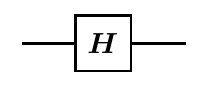
\includegraphics[scale=0.4]{images/hadamard_gate.png}
\end{center}
and the two-qubit {\it controlled phase gate} $\Lambda(\mathbf{P})$ acts in the canonical basis $\{\ket{00},\ket{01},\ket{10},\ket{11}\}$
as the diagonal $4\times 4$ matrix
\begin{equation}
\Lambda(\mathbf{P}) = \text{diag}(1,1,1,i)
\end{equation}
and can be denoted by
\begin{center}
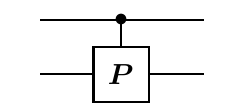
\includegraphics[scale=0.4]{images/cphase_gate.png}
\end{center}
\begin{enumerate}[a)]
\item Consider the two-qubit unitary transformations $U_1$ and $U_2$ defined by the quantum circuits
\begin{center}
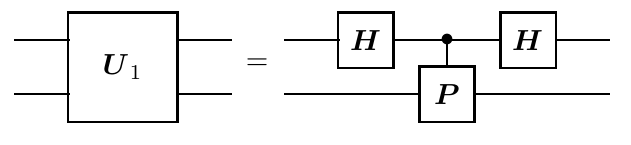
\includegraphics[scale=0.4]{images/u1.png}
\end{center}
and
\begin{center}
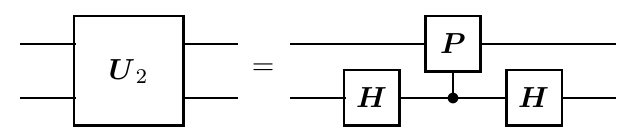
\includegraphics[scale=0.4]{images/u2.png}
\end{center}
Let $\ket{ab}$ denote the element of the standard basis where $a$ labels the upper qubit in the circuit diagram
and $b$ labels the lower qubit. Show that $U_1$ and $U_2$ both act trivially on the states
\begin{equation}
\ket{00}, \quad \frac{1}{\sqrt 3}\left(\ket{01} + \ket{10} + \ket{11}\right)
\end{equation}

\item Thus $U_1$ and $U_2$ act nontrivially only in the two-dimensional space spanned by
\begin{equation}
\left\{ \ket{\phi_1} = \frac{1}{\sqrt 2}\left(\ket{01}-\ket{10}\right), \quad \ket{\phi_2} = \frac{1}{\sqrt 6}\left(\ket{01} + \ket{10} - 2\ket{11}\right) \right\}.
\end{equation}
Find $U_1$ and $U_2$ in this basis.
\end{enumerate}

\Problem 2
What is the effect of the quantum circuit depicted in Fig.\ 1
on the initial states $\ket{00}$, $\ket{01}$, $\ket{10}$, $\ket{11}$?
\begin{figure}[h!]
\centering
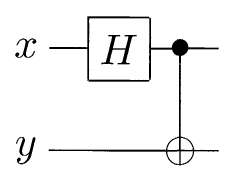
\includegraphics[scale=0.44]{images/epr_gate.png}
\caption{Quantum circuit}
\end{figure}


\Problem 3
Suppose Alice wants to send Bob two bits of classical information. Initially,
they share an entangled qubit in the state
\begin{equation}
\ket{\psi_0} = \frac{1}{\sqrt 2} \left( \ket{00} + \ket{11} \right).
\end{equation}
Alice performs any operation on her qubit and then sends it to Bob. How can she send
two bits of classical information to Bob?

\end{document}
